\section{Validation of the Estimator and of the Intervals}
\label{sec:validation}
\label{sec:validation_estimator}
Toy-MC experiments generated from the fitted model of Sec.~\ref{sec:model} (Poisson yields, masses drawn from the model; $1000$ at the fitted value $A_{\mathrm{true}}=-0.0441$ and $300$ at each of $-0.1$, $-0.02$, $0$ and $+0.05$, $1$--$3\%$ of the fits not valid and excluded) verify the estimator and the profile-likelihood ratio\appref{app:ext_valid}. The bias of $\hat A$ is at most $0.0008$ ($1.6$ standard errors; $-0.0005$, $-0.0001$, $-0.0008$, $+0.0002$, $-0.0004$ for the five values), its spread equals the mean Hesse uncertainty within $6\%$ and the pulls have width $0.94$--$1.05$: the estimator is unbiased and reaches the minimum variance bound.

At the fitted value the coverage of $t(A_{\mathrm{true}})\leq1$ is $0.696\pm0.015$ ($68.3\%$ level) and $0.954\pm0.007$ ($95.4\%$ level); the $68\%$ coverage over the five values is $0.71$, $0.70$, $0.69$, $0.69$ and $0.61$, the last, at $+0.05$ ($0.614\pm0.028$), $2.5$ standard deviations low, not unexpected among five values.

Inverting the Neyman construction of the same experiments (Fig.~\ref{fig:checks_belt}) at the observed $\hat A$\appref{sec:checks_belt} gives the $68\%$ interval $[-0.0528,-0.0351]$, against the Minos interval $[-0.0526,-0.0356]$.

Under $A_{\mathrm{true}}=0$ the test $q(0)>3.84$ rejects in $0.051\pm0.013$ of the experiments, the nominal size, with $q(0)$ compatible with $\chi^2_1$ (Kolmogorov-Smirnov $p=0.79$); its power is $1.00$ at the fitted value and $0.68$ ($0.27$ at $3\sigma$) at $A_{\mathrm{true}}=-0.02$, so with $19{,}731$ candidates an asymmetry below $\sim0.02$ is not resolved\appref{sec:validation_power}. The $5.2\sigma$ of the data is an extrapolation of the $\chi^2_1$ tail, which the $293$ experiments check only down to the $3\sigma$ level.

\begin{figure}[h]
\centering
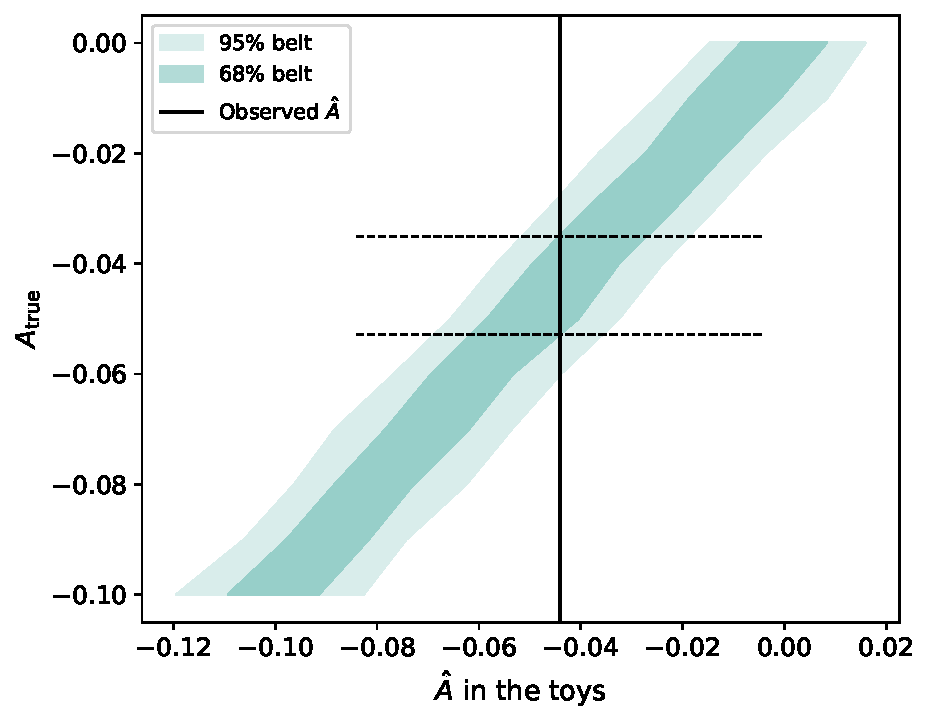
\includegraphics[width=\columnwidth]{figures/validation_neyman_belt.pdf}
\caption{Confidence belt of $\hat A$ from toy-MC experiments (central $68\%$ and $95\%$ ranges) as a function of $A_{\mathrm{true}}$; the vertical line is the observed $\hat A$ and the dashed lines the resulting $68\%$ interval.}
\label{fig:checks_belt}
\end{figure}
